\chapter{Studi Literatur}
\label{chapter:studi-literatur}

Bab ini akan diisi oleh studi literatur yang terkait dengan topik persoalan pada tugas akhir untuk memberikan informasi mengenai dasar teori dan literatur yang digunakan. Bab ini diharapkan dapat membantu pembaca memiliki pengetahuan yang menyeluruh dan dasar yang cukup untuk mengerti penelitian ini.

\section{Blockchain}

\textit{Blockchain} adalah sekuens dari blok yang menyimpan daftar transaksi lengkap seperti \textit{public ledger} konvensional, dimana setiap \textit{ledger} disimpan pada \textit{node} yang tersebar seperti pada \textit{Distributed Ledger Technology} \parencite{zheng2018blockchain}. Setiap transaksi yang masuk ke dalam sebuah blok akan divalidasi sesuai dengan metrik yang digunakan oleh sistem \textit{blockchain}, dan blok yang memiliki daftar transaksi yang lengkap, ditambah \textit{timestamp} pembuatan blok, nilai \textit{hash} dari blok sebelumnya ("\textit{parent}"), dan sebuah \textit{nonce}, yang adalah sebuah angka acak yang digunakan untuk mekanisme verifikasi \textit{hash}. Konsep ini memastikan integritas dari \textit{blockchain} dimulai dari blok pertama ("\textit{genesis block}") sampai ke blok terakhir, yang terus ditambahkan, karena setiap perubahan data akan membuat nilai \textit{hash} dari sebuah blok berubah, yang harus dipropagasikan ke setiap blok setelahnya. Sebelum ditambahkan ke dalam \textit{blockchain}, setiap blok dan transaksi di dalamnya harus divalidasi oleh mayoritas \textit{node}, menggunakan sebuah mekanisme \textit{consensus} \parencite{nofer2017blockchain}. Mekanisme \textit{consensus} adalah proses dimana mayoritas dari \textit{network validator} menyetujui atau menolak sebuah \textit{state} dari \textit{ledger}. Proses \textit{consensus} mengikuti sebuah kumpulan aturan dan prosedur untuk mempertahankan himpunan fakta yang koheren diantara beberapa \textit{participating nodes}. Terdapat banyak mekanisme \textit{consensus} yang berbeda yang digunakan dalam \textit{blockchain network} yang berbeda. Dalam kasus \textit{Bitcoin}, \textit{ledger} yang dianggap \textit{ledger} yang \textit{valid} adalah \textit{ledger} dengan \textit{chain} terpanjang (\textit{longest chain}) \parencite{swanson2015consensus}.

\begin{figure}[ht]
	\centering
	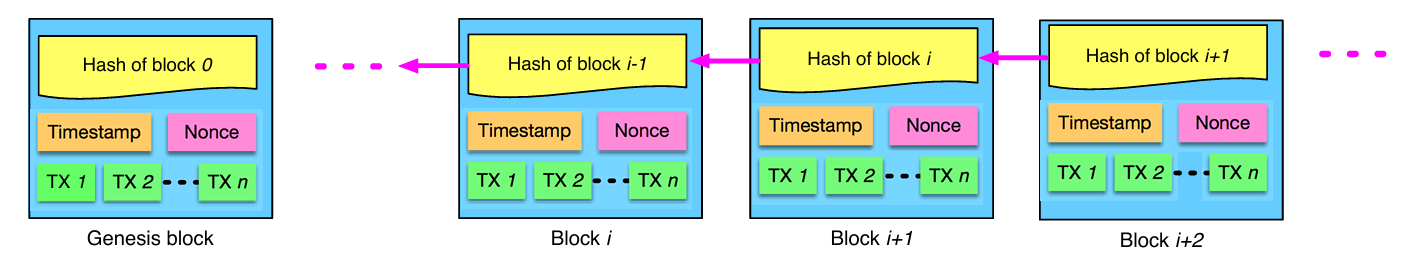
\includegraphics[width=1\textwidth]{resources/chapter-2/struktur-blockchain.png}
	\caption{Struktur blok di dalam \textit{blockchain} \parencite{zheng2018blockchain}}
	\label{image:struktur-blockchain}
\end{figure}

\break

Struktur dari sebuah blok terdiri dari \textit{block header} dan \textit{block body} seperti pada gambar \ref{image:struktur-blok}. Secara spesifik, \textit{block header} terdiri dari:

\begin{enumerate}
	\item \textit{Block Version}: mengindikasikan set dari aturan validasi yang diikuti.
	\item \textit{Parent Block Hash}: 256-bit \textit{hash} dari blok sebelumnya.
	\item \textit{Merkle Tree Root}: hasil \textit{hash} dari seluruh transaksi pada blok menggunakan mekanisme \textit{Merkle Tree}.
	\item \textit{Timestamp}: \textit{timestamp} saat ini dalam detik sejak 1970-01-01T00:00 UTC.
	\item \textit{nBits}: target \textit{hash} saat ini dalam format \textit{compact}.
	\item \textit{nonce}: \textit{number used only once}, sebuah angka yang digunakan untuk menambahkan tingkat keacakan dari nilai \textit{hash}.
\end{enumerate}

\begin{figure}
	\centering
	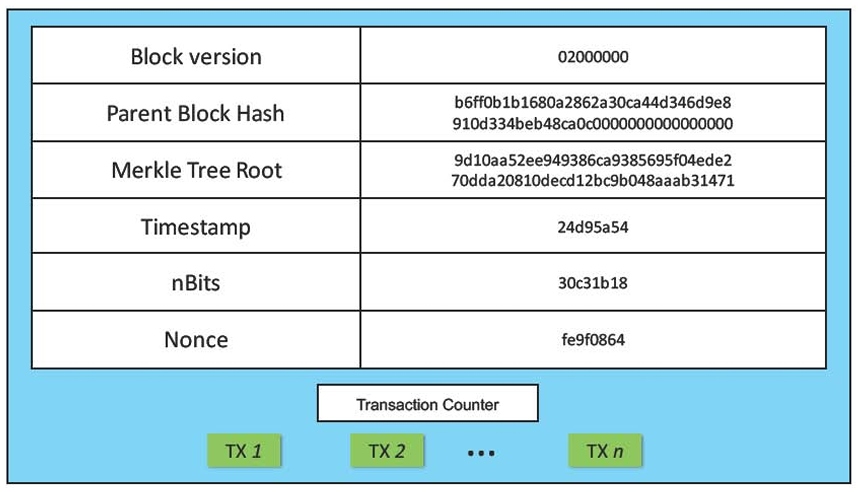
\includegraphics[width=0.7\textwidth]{resources/chapter-2/struktur-block.png}
	\caption{Struktur blok \parencite{zheng2018blockchain}}
	\label{image:struktur-blok}
\end{figure}



% \subsection{Contoh Subsubbab}
% \label{subsec:contoh-subsec}



% \subsubsection{Subsubsubbab}
% \blindtext

% \subsubsubsection{sub sub sub sub bab}
% \blindtext

% \begin{table}[h]
% 	\caption{Tabel random}
% 	\vspace{0.25cm}
% 	\begin{center}
% 		\begin{tabular}{|c|c|c|c|}
% 			\hline
% 			Title1 & Title2 & Title3 & Title4  \tabularnewline
% 			\hline
% 			1647   & 1.97   & 0.68   & 1.90 \tabularnewline
% 			2301   & 2.92   & 1.06   & 2.75 \tabularnewline
% 			2969   & 3.23   & 1.16   & 3.78 \tabularnewline
% 			3791   & 4.39   & 1.40   & 4.14 \tabularnewline
% 			4625   & 6.72   & 1.87   & 5.59 \tabularnewline
% 			\hline
% 		\end{tabular}
% 	\end{center}
% \end{table}
\section{Smart Contracts}
\label{sec:smart-contract}

Smart Contracts adalah sebuah protokol transaksi elektronik yang mengeksekusi kesepakatan dari sebuah kontrak. Klausa kesepakatan yang dimasukkan ke dalam sebuah Smart Contract akan diberlakukan secara otomatis saat kondisi yang sesuai sudah tercapai. Sehingga, suatu pihak yang melanggar kontrak akan dihukum secara otomatis. Smart Contract adalah sebuah cara untuk meminimalisir kepercayaan kepada perantara pihak ketiga sebagai \textit{enforcer} dari sebuah kontrak \parencite{szabo1997formalizing}.

Smart Contracts adalah salah satu teknologi yang dimungkinkan oleh teknologi Blockchain. Seluruh klausa kontraktual dalam sebuah Smart Contract akan dikonversi menjadi sebuah bentuk \textit{executable computer programs}. Seluruh eksekusi dari setiap \textit{contract statement} direkam dan dimasukkan ke dalam transaksi yang \textit{immutable}, yang disimpan di dalam Blockchain. Smart Contracts juga dapat menjamin \textit{access control} yang tepat dan \textit{contract enforcement} yang deterministik, karena dijamin dalam seluruh \textit{logic} yang terdapat di dalam Smart Contract tersebut \parencite{zheng2020overview}.

\begin{figure}[ht]
	\centering
	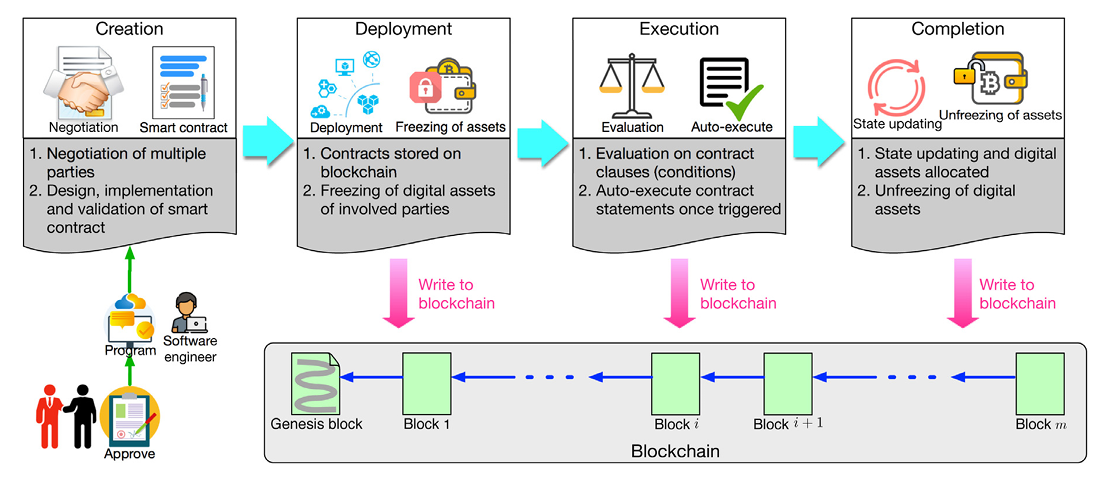
\includegraphics[width=0.7\textwidth]{resources/chapter-2/sc-lifecycle.png}
	\caption{\textit{Life cycle} dari Smart Contract \parencite{zheng2020overview}}
	\label{image:sc-lifecycle}
\end{figure}

\textit{Life cycle} dari sebuah Smart Contract terdiri dari empat fase seperti pada ilustrasi di Gambar \ref{image:sc-lifecycle}:

\begin{enumerate}
	\item \textit{Creation}: negosiasi antar pihak untuk menyepakati ketentuan dari kontrak dalam \textit{natural language}, dan translasi menjadi Smart Contracts.
	\item \textit{Deployment}: kontrak yang sudah divalidasi dapat disimpan ke dalam Blockchain, menjadikannya tidak bisa dimodifikasi.
	\item \textit{Execution}: Setelah \textit{deployment}, klausa kontraktual akan dimonitor, dan saat kondisi yang sesuai dengan yang terdefinisi dalam Smart Contract, maka prosedur kontrak akan dieksekusi secara otomatis.
	\item \textit{Completion}: Setelah eksekusi, \textit{state} baru dari semua pihak akan diperbarui sesuai dengan hasil dari transaksi yang terjadi dan disimpan ke dalam Blockchain. 
\end{enumerate}

\subsection{Off-Chain Smart Contracts}
\label{subsec:off-chain-smart-contracts}

\textit{Off-chain Smart Contract} adalah Smart Contracts yang dieksekusi diluar Blockchain, \textit{signed} hanya oleh \textit{interested participants}, dan digunakan untuk mengenkapsulasi fungsi yang melibatkan komputasi \textit{high-cost} atau \textit{private information} terkait \textit{participants}. Terdapat banyak cara untuk tetap menjaga properti dan keuntungan penggunaan dari Blockchain, contohnya, hasil dari eksekusi sebuah \textit{off-chain Smart Contract} dapat dilakukan \textit{logging} pada Blockchain, sehingga jika terjadi \textit{dispute} dalam eksekusi \textit{off-chain Smart Contract}, sebuah \textit{on-chain Smart Contract} dappat digunakan untuk \textit{fork off-chain Smart Contract} dan mengeksekusinya di dalam Blockchain untuk menyelesaikan \textit{dispute} \parencite{zou2019smart}.

\subsection{Semantic Smart Contracts}
\label{subsec:semantic-smart-contracts}
\textit{Semantic Smart Contracts} adalah sebuah cara untuk merepresentasikan \textit{semantics} dari Smart Contract menggunakan konsep \textit{EthOn contract extension} dan sebuah \textit{vocabulary} yang terkait dengan bisnis. \textit{Semantic Smart Contracts} mengizinkan untuk membandingkan \textit{request} dengan beberapa \textit{request description} dengan mengonsiderasi semantik dari anotasi yang mereferensikan sebuah \textit{shared domain ontology} \parencite{baqa2019semantic}.

\section{Ontology}
\label{sec:ontology}

Pada tahun 1993, \cite{gruber1993translation} pertama mendefinisikan sebuah \textit{ontology} sebagai "\textit{explicit specification of a conceptualization}". Pada tahun 1997, \cite{borst1997construction} mendefinisikan \textit{ontology} sebagai "\textit{formal specification of a shared conceptualization}". Definisi ini menambahkan kebutuhan sebuah \textit{ontology} sebagai sebuah representasi konseptual yang \textit{shared} diantara beberapa pihak. Sehingga, konseptualisasi tersebut harus diekspresikan dengan sebuah format yang \textit{machine readable}. Sehingga pada tahun 1998, \cite{studer1998knowledge} menggabungkan kedua definisi tersebut sebagai "\textit{an ontology is a formal, explicit specification of a shared conceptualization}."

Dalam tulisannya, \cite{Guarino2009} merangkum ketiga definisi tersebut menjadi: \textit{Ontology} adalah sebuah \textit{framework} terstruktur untuk merepresentasikan pengetahuan di sebuah \textit{domain} tertentu, seperti mendefinisikan entitas, konsep, dan relasi di dalam \textit{domain} tersebut. \textit{Ontology} dapat membantu membuat sebuah model yang dapat dimengerti dan dapat dibagikan untuk digunakan dalam berbagai sistem dan aplikasi. Di dalam \textit{domain} sistem informasi, \textit{ontology} digunakan sebagai sebuah cara formal untuk mengorganisasikan dan merepresentasikan data untuk dibagikan, dilakukan pencarian, dan dilakukan penalaran \parencite{Guarino2009}. 

Beberapa komponen kunci dari sebuah \textit{ontology} adalah:

\begin{enumerate}
  \item \textit{Classes (Concepts)}: Tipe atau kategori fundamental di dalam sebuah \textit{domain} yang merepresentasikan konsep umum.
  \item \textit{Instances (Individuals)}: Contoh spesifik dari sebuah \textit{class}.
  \item \textit{Properties (Attributes)}: Mendeskripsikan karakteristik dari \textit{classes} atau \textit{instances}.
  \item \textit{Relationships}: Hubungan antar entitas, bisa \textit{hierarchical} atau \textit{associative}.
  \item \textit{Axioms}: Aturan atau \textit{constraint} yang mendefinisikan \textit{valid relationships} dan \textit{properties} di dalam \textit{ontology}, sehingga dapat dilakukan inferensi logis.
\end{enumerate}

\subsection{The Semantic Web}
\label{subsec:the-semantic-web}

\textit{The Semantic Web} adalah sebuah ekstensi dari \textit{web} dengan tambahan data dengan arti yang terdefinisi dengan baik, yang diturunkan menggunakan \textit{semantic theory} untuk menginterpretasikan simbol-simbol. \textit{Semantic theory} menyediakan catatan dari arti untuk sebuah istilah atau informasi, sehingga dapat membuat sebuah hubungan logis antar istilah \parencite{shadbolt2006semantic}.

\subsubsection{Universal Resource Identifiers}
\label{subsubsec:universal-resource-identifiers}

\textit{Universal Resource Identifiers (URIs)} adalah sebuah cara untuk mengidentifikasi sebuah \textit{resource} menggunakan sebuah konvensi penamaan global yang disepakati, sehingga dapat diinterpretasikan secara standar oleh seluruh mesin yang berada di \textit{web}. Saat sebuah \textit{resource} diasosiasikan dengan sebuah URI, maka itu berarti semua orang dapat melakukan \textit{link}, \textit{refer}, dan mengambil \textit{representasi} dari \textit{resource} tersebut menggunakan URI. Skema yang direkomendasikan pada tahun 2004 adalah \textit{Resource Definition Framework Schema} yang menggunakan spesifikasi dasar dari RDF dengan ekstensi untuk mendukung ekspresi dari \textit{structured vocabularies} \parencite{shadbolt2006semantic}.

\subsubsection{Web Ontology Langugage}
\label{subsubsec:web-ontology-language}

\textit{Web Ontology Language (OWL)} adalah keluarga bahasa yang dikembangkan oleh \textit{World Wide Web Consortium (W3C)}, digunakan untuk mengembangkan dan berbagi \textit{ontology} di dalam \textit{web}. OWL bertujuan untuk memberikan representasi yang efisien untuk \textit{ontology}, pengecekan \textit{logical consistency} dan klasifikasi \textit{concept}, menggunakan RDF untuk \textit{linking} sehingga \textit{ontology} dapat didistribusikan antar sistem \parencite{shadbolt2006semantic}.


% Bab Studi Literatur digunakan untuk mendeskripsikan kajian literatur yang terkait dengan persoalan tugas akhir. Tujuan studi literatur adalah:

% \begin{enumerate}
% 	\item menunjukkan kepada pembaca adanya gap seperti pada rumusan masalah yang memang belum terselesaikan,
% 	\item memberikan pemahaman secukupnya kepada pembaca tentang teori atau pekerjaan terkait yang terkait langsung dengan penyelesaian persoalan, serta
% 	\item menyampaikan informasi apa saja yang sudah ditulis/dilaporkan oleh pihak lain (peneliti/Tugas Akhir/Tesis) tentang hasil penelitian/pekerjaan mereka yang sama atau mirip kaitannya dengan persoalan tugas akhir.
% \end{enumerate}

% Kita juga dapat memisah beberapa bagian latex untuk \textit{readability}. Kita dapat memasukan file latex lainnya dengan menggunakan fitur input. Berikut merupakan contoh ketika memasukan bagian contoh-subbab ke chapter-2


% \section{Menyisipkan Persamaan}

% Beberapa contoh menyisipkan persamaan.

% \subsection{Contoh Bikin Equation}
% \textbf{text tebal} dan ini \emph{miring}, bikin persamaan di baris yang sama, tinggal pake dolar2 $\Psi(\vec{r}_1,...,\vec{r}_N)$, sehingga persamaan Schr\"{o}dinger, terus, persamaan yang dinomeri kayak gini
% %ini contoh bikin persamaan, ..... :D
% \begin{equation}
% 	\left[ \sum_{i}^{N}-\frac{\hbar^2}{2m}\nabla_i^2 + \sum_{i}^{N}V(\vec{r}_i)+ \sum_{i<j}^{N}(\vec{r}_i,\vec{r}_j)\right]\Psi = E\Psi
% \end{equation}

% untuk $N$-elektron, dengan $\hat{H}$=Hamiltonian, $E$=Energi total, $\hat{T}$=Energi kinetik, $\hat{V}$=Energi potensial, dan $\hat{U}$=Interaksi ektron-elektron.

% \subsection{Bikin Matrix}
% Lalalallala.... bikin matrix sekarang, yang ini dikecilin, pake smaller
% 	{\smaller
% 		\begin{equation}
% 			\Psi({\bf r}_1, {\bf r}_2, \cdots {\bf r}_N) = \frac{1}{\sqrt{N!}}\left| \begin{array}{llcl}
% 				\phi_1({\bf r}_1)     & \phi_2({\bf r}_1)     & \cdots                & \phi_N({\bf r}_1)     \\
% 				\phi_1({\bf r}_2)     & \phi_2({\bf r}_2)     & \cdots                & \phi_N({\bf r}_2)     \\
% 				\phi_1({\bf r}_3)     & \phi_2({\bf r}_3)     & \cdots                & \phi_N({\bf r}_3)     \\
% 				\multicolumn{1}{c}{.} & \multicolumn{1}{c}{.} & \multicolumn{1}{c}{.} & \multicolumn{1}{c}{.} \\
% 				\multicolumn{1}{c}{.} & \multicolumn{1}{c}{.} & \multicolumn{1}{c}{.} & \multicolumn{1}{c}{.} \\
% 				\multicolumn{1}{c}{.} & \multicolumn{1}{c}{.} & \multicolumn{1}{c}{.} & \multicolumn{1}{c}{.} \\
% 				\phi_1({\bf r}_N)     & \phi_2({\bf r}_N)     & \cdots                & \phi_N({\bf r}_N)     \\
% 			\end{array} \right|
% 		\end{equation}
% 	}